% Idee: ???
% Tekst: ???
% Tõlge: Katrin Gabrel, Ahto Truu

\documentclass[a4paper,11pt]{article}
\usepackage[et]{../../eio}

\usepackage{tikz}
\tikzset{every picture/.style = {thick, scale=0.5}}
\tikzset{uno/.style = {fill, shape=circle, inner sep=2}}
\tikzset{post/.style = {fill, shape=circle, inner sep=1}}
\tikzset{label/.style = {black, midway}}

\begin{document}

\begin{ol}{\eio}{\vv 19.04.2020}{\yle}{}
\begin{yl}{1}{Aed}{aed}{1 sek / 3 sek}{100 punkti}

Onu Uno ehitab karjamaa ümber aeda. Aed on $N$ sirglõigust koosnev kinnine murdjoon. See tähendab, et iga järgmine lõik algab sealt, kus eelmine lõppes, ja viimane lõik lõpeb esimese lõigu alguspunktis. Lõigud on nummerdatud $1 \ldots N$ vastupäeva. Võib eeldada, et aialõigud omavahel ei lõiku ega puutu (välja arvatud järjestikuste lõikude ühised otspunktid).

Kui Onu Uno on aia valmis saanud, tahab ta selle üle vaadata. Kirjuta programm, mis saab Onu Uno asukoha ja leiab, milliseid aialõike ta seal seistes näeb. Onu Uno võib seista nii aia sees kui ka sellest väljas, kuid mitte ühegi aialõiguga samal sirgel.

Onu Uno näeb aialõiku, kui leidub tema asukohta ja aialõigu mingit punkti ühendav sirglõik, mis ei lõika ega puutu ühtegi teist aialõiku. (Teisisõnu, aialõigu Unole nähtav osa peab olema nullist suurema pikkusega.)

\sis Tekstifaili \sisf esimesel real on aialõikude arv $N$ ($3 \le N \le 1\,000$). Teisel real on kaks tühikuga eraldatud täisarvu: Onu Uno asukoha koordinaadid $X$ ja $Y$. Järgmisel $N$ real on igaühel kaks tühikuga eraldatud täisarvu: real $i + 2$ on aialõigu number $i$ alguspunkti koordinaadid $X_i$ ja $Y_i$. Kõik koordinaadid on täisarvud absoluutväärtusega kuni $10^5$.

\val Tekstifaili \valf esimesele reale väljastada üks täisarv: Onu Unole nähtavate aialõikude arv $M$. Teisele reale väljastada $M$ tühikutega eraldatud täisarvu: nähtavate aialõikude numbrid kasvavas järjekorras.

\begin{wrapfigure}[1]{r}{0.3\textwidth}
\vskip -20pt
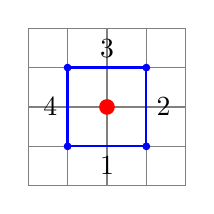
\begin{tikzpicture}
  \draw[gray, thin, step=1] (0, 0) grid (4, 4);
  \draw[blue] (1, 1)
    -- (3, 1) node[post]{} node[label, below]{1}
    -- (3, 3) node[post]{} node[label, right]{2}
    -- (1, 3) node[post]{} node[label, above]{3}
    -- (1, 1) node[post]{} node[label, left]{4};
  \fill[red] (2, 2) node[uno]{};
\end{tikzpicture}
\vskip 10pt
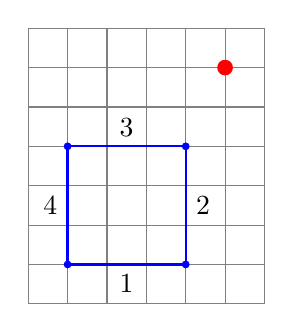
\begin{tikzpicture}
  \draw[gray, thin, step=1] (0, 0) grid (6, 7);
  \draw[blue] (1, 1)
    -- (4, 1) node[post]{} node[label, below]{1}
    -- (4, 4) node[post]{} node[label, right]{2}
    -- (1, 4) node[post]{} node[label, above]{3}
    -- (1, 1) node[post]{} node[label, left]{4};
  \fill[red] (5, 6) node[uno]{};
\end{tikzpicture}
\vskip 10pt
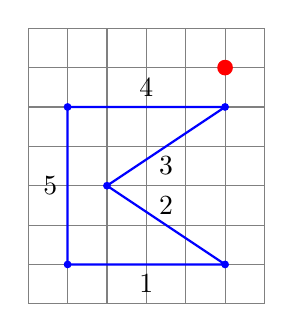
\begin{tikzpicture}
  \draw[gray, thin, step=1] (0, 0) grid (6, 7);
  \draw[blue] (1, 1)
    -- (5, 1) node[post]{} node[label, below]{1}
    -- (2, 3) node[post]{} node[label, above]{2}
    -- (5, 5) node[post]{} node[label, below]{3}
    -- (1, 5) node[post]{} node[label, above]{4}
    -- (1, 1) node[post]{} node[label, left]{5};
  \fill[red] (5, 6) node[uno]{};
\end{tikzpicture}
\end{wrapfigure}

\nde[0]{3cm}{3cm}

\nde[1]{3cm}{3cm}

\nde[2]{3cm}{3cm}

\hnd Selles ülesandes on testid jagatud gruppidesse. Iga grupi eest saavad punkte ainult need lahendused, mis läbivad kõik sellesse gruppi kuuluvad testid. Gruppides kehtivad järgmised lisatingimused:
\begin{xitem}
  \item ($3 + 3$ punkti) $N \le 50$ ja aed moodustab kumera hulknurga;
  \item ($7 + 7$ punkti) aed moodustab kumera hulknurga;
  \item ($2 + 5 + 5$ punkti) $N \le 50$ ja aia kõik lõigud on paralleelsed kas X- või Y-teljega;
  \item ($18$ punkti) aia kõik lõigud on paralleelsed kas X- või Y-teljega;
  \item ($4 + 5 + 5$ punkti) $N \le 50$;
  \item ($16$ punkti) $N \le 200$;
  \item ($20$ punkti) lisapiirangud puuduvad.
\end{xitem}

\end{yl}
\end{ol}
\end{document}
